\documentclass{beamer}
\usepackage[utf8]{inputenc}
\usepackage{listings}
\usepackage{pgffor}
\usepackage{minted}
\usepackage{array}
\usepackage{tikz}
\usetikzlibrary{angles,quotes}
% \usepackage[style=ieee]{biblatex}
% \usepackage{unicode-math}
\usepackage[prefix=]{xcolor-material}
\usetheme{seville}
\definecolor{buttonback}{HTML}{083444}
\makeatletter
\defbeamertemplate*{frametitle continuation}{only if multiple}{%
    \ifnum \numexpr\beamer@endpageofframe+1-\beamer@startpageofframe\relax > 1
        \textmd{(%
            \insertcontinuationcount/%
            \the\numexpr\beamer@endpageofframe+1-\beamer@startpageofframe%
        )}%
    \fi%
}
\makeatother

\newcolumntype{C}[1]{>{\centering\arraybackslash}m{#1}}
\newcolumntype{L}[1]{>{\raggedright\arraybackslash}m{#1}}
\newcolumntype{N}{@{}m{0pt}@{}}

\setbeamercolor{button}{bg=buttonback,fg=Amber50!85!Grey}

% \addbibresource{demo.bib}

\title{Simuler les feux de forêt}
\subtitle{Comment utiliser l'informatique pour réduire l'impact des feux de forêts en transformant le moins possible ces dernières ?}
\author{Victor Sarrazin}
\date{N° SCEI 14423}

\setbeamertemplate{footline}{%
  \raisebox{10pt}{% 
    \makebox[\paperwidth]{%
      \hfill\makebox[20pt]{%
        \large\textbf\insertframenumber 
      }
    }
  }
}

\begin{document}
% \setmathfont{TeX Gyre Schola Math}

\begin{frame}[noframenumbering,plain]

    \titlepage

\end{frame}

\begin{frame}
    \frametitle{Introduction \hyperlink{jump}{\beamerbutton{ }} \hypertarget{1}{\beamerbutton{ }}}

    \begin{block}{Contexte}
        Les feux de forêt sont de plus en plus fréquents. L'informatique peut se révéler être un atout de taille pour prévoir et anticiper ces derniers.
    \end{block}

    \begin{figure}
        \centering
        \includegraphics[width=0.5\linewidth]{pictures/intro.jpg}
        \caption{Feu de forêt à Malibu\footnote{National Geographic Education}}
        \label{fig:enter-label}
    \end{figure}
\end{frame}


\section{Un premier modèle de feux de forêt}
\section{Modèle d'Alexandridis pour les feux de forêt}
\section{Étude des transformations réalisables}

\begin{frame}{Sommaire \hyperlink{jump}{\beamerbutton{ }} \hypertarget{2}{\beamerbutton{ }}}
    \tableofcontents
\end{frame}

\begin{frame}{Un premier modèle de feux de forêt \hyperlink{jump}{\beamerbutton{ }} \hypertarget{3}{\beamerbutton{ }}}
    \begin{block}{Automate cellulaire (2D)}
        \begin{itemize}
            \item Une grille
            \item Un état par case
            \item Un ensemble de règles de transitions entre les états
        \end{itemize}
    \end{block}

    \begin{figure}
        \centering
        \includegraphics[width=0.25\linewidth]{pictures/moore.png}
        \caption{Voisinage de Moore {\footnote{Science Direct}}}
        \label{fig:enter-label}
    \end{figure}
\end{frame}

\begin{frame}{Un premier modèle de feux de forêt \hyperlink{jump}{\beamerbutton{ }} \hypertarget{4}{\beamerbutton{ }}}
    \begin{block}{Types de cases :}
        \begin{itemize}
            \item Arbres
            \item Champs
            \item Feu
            \item Case brulée *
            \item Eau *
        \end{itemize}

        * Ne peuvent pas/plus bruler
    \end{block}

    \begin{figure}
        \begin{center}
            \renewcommand{\arraystretch}{2}
            \setlength{\extrarowheight}{-3pt}
            \begin{table}
                \begin{tabular}{ |C{2cm}|L{3cm}|C{3cm}|N }
                \hline
                $p_{b}$ & Voisin direct & Voisin diagonal \\
                \hline 
                Arbres & \centering $\tfrac{1}{8}$ & $\tfrac{1}{16}$ \\ 
                \hline
                Champs & \centering $\tfrac{1}{8}$ & $\tfrac{1}{16}$ \\
                \hline 
                \end{tabular}
            \end{table}
        \end{center}
        \caption{Probabilité de changement d'état}
    \end{figure}
\end{frame}

\begin{frame}{Un premier modèle de feux de forêt \hyperlink{jump}{\beamerbutton{ }} \hypertarget{5}{\beamerbutton{ }}}
    \begin{figure}[!htb]
        \begin{minipage}{0.48\textwidth}
          \centering
          \includegraphics[width=.8\linewidth]{pictures/model1/land_before.png}
          \caption{À $t=0$}\label{Fig:Data1}
        \end{minipage}\hfill
        \begin{minipage}{0.48\textwidth}
          \centering
          \includegraphics[width=.8\linewidth]{pictures/model1/land_200.png}
          \caption{À $t=200$}\label{Fig:Data2}
        \end{minipage}
     \end{figure}
\end{frame}

\begin{frame}{Vers le modèle d'Alexandridis \hyperlink{jump}{\beamerbutton{ }} \hypertarget{6}{\beamerbutton{ }}}
    \begin{block}{Idée}
        Il serait intéressant de prendre en compte des données du milieu : vent, densité de végétation
    \end{block}
\end{frame}

\begin{frame}{Modèle d'Alexandridis pour les feux de forêt \hyperlink{jump}{\beamerbutton{ }} \hypertarget{7}{\beamerbutton{ }}}
    \begin{block}{Nouveau type de case :}
        \begin{itemize}
            \item Arbres denses
        \end{itemize}
    \end{block}

    \hspace{1cm}

    \begin{block}{Règles de transition}
        Pour tout $(i,j,t) \in \mathbb{N}^3$, on a :
        \begin{itemize}
            \item Si $m_{i,j} (t) = $ \mintinline{latex}{feu} alors $m_{i,j} (t+1) = $ \mintinline{latex}{brulé}
            \item Si $m_{i,j} (t) = $ \mintinline{latex}{feu} alors $m_{i \pm 1,j \pm 1} (t+1) = $ \mintinline{latex}{feu} avec une probabilité $p_b$
            \item Si $m_{i,j} (t) = $ \mintinline{latex}{brulé} alors $m_{i,j} (t+1) = $ \mintinline{latex}{brulé}
        \end{itemize}
    \end{block}
\end{frame}

\begin{frame}{Modèle d'Alexandridis pour les feux de forêt \hyperlink{jump}{\beamerbutton{ }} \hypertarget{8}{\beamerbutton{ }}}
    \begin{block}{Probabilité d'inflammation $p_b$}
        On a $p_b = p_h (1 + p_{veg}) (1 + p_{den}) p_{vent}$ avec $p_h = 0.27$ une constante
    \end{block}

    Plus la végétation est dense, plus $p_{den}$ est élevée
    Plus la végétation a du combustible, plus $p_{veg}$ est élevée

    \begin{figure}[!h]
        \centering
        \renewcommand{\arraystretch}{2}
        \setlength{\extrarowheight}{-3pt}
        \begin{tabular}{ |>{\centering\arraybackslash}p{4cm}|>{\centering\arraybackslash}p{2cm}|>{\centering\arraybackslash}p{2cm}| }
            \cline{2-3}
            \multicolumn{1}{c|}{} & $p_{veg}$ & $p_{den}$ \\
            \hline 
            Arbres & $0.3$ & $0$ \\ 
            \hline
            Arbres denses & $0.3$ & $0.3$ \\ 
            \hline
            Champs & $-0.1$ & $0$ \\
            \hline 
        \end{tabular}
        \caption{Probabilités $p_{veg}$ et $p_{den}$ selon le type de végétation}
    \end{figure}
\end{frame}

\begin{frame}{Modèle d'Alexandridis pour les feux de forêt \hyperlink{jump}{\beamerbutton{ }} \hypertarget{9}{\beamerbutton{ }}}
    \begin{block}{Probabilité liée au vent $p_{vent}$}
        On a $p_{vent} = exp(0.045 v) \times exp (0.131 v \times (cos(\theta) - 1))$ avec $\theta$ l'angle entre la propagation du feu et la direction du vent et $v$ la vitesse du vent (en $m/s$)
    \end{block}

    \vspace{30px}

    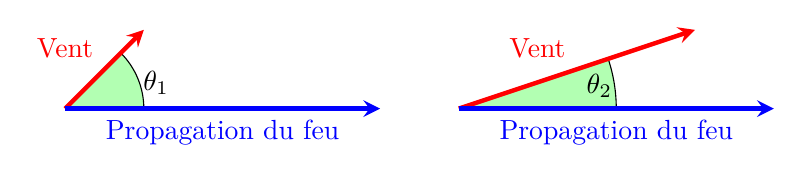
\begin{tikzpicture}[> = stealth]
        \coordinate (a) at (1,4);
        \coordinate (b) at (2,5);
        \coordinate (c) at (5,4);
        \coordinate (d) at (6,4);
        \coordinate (e) at (9,5);
        \coordinate (f) at (10,4);
        
        \draw pic[draw,fill=green!30,angle radius=1cm,"$\theta_1$" shift={(6mm,1mm)}] {angle=c--a--b};
        \draw pic[draw,fill=green!30,angle radius=2cm,"$\theta_2$" shift={(6mm,1mm)}] {angle=f--d--e};
        
        \draw[ultra thick,red, ->]  (a) -- node[above left] {\normalsize Vent} (b);
        \draw[ultra thick,blue,->]  (a) -- node[below] {\normalsize Propagation du feu} (c);

        \draw[ultra thick,red, ->]  (d) -- node[above left] {\normalsize Vent} (e);
        \draw[ultra thick,blue,->]  (d) -- node[below] {\normalsize Propagation du feu} (f);
        \end{tikzpicture}
\end{frame}

\begin{frame}{Modèle d'Alexandridis pour les feux de forêt \hyperlink{jump}{\beamerbutton{ }} \hypertarget{10}{\beamerbutton{ }}}
    Comparaison du premier modèle et de celui d'Alexandridis à $t=200$.
    
    \begin{figure}[!htb]
        \begin{minipage}{0.48\textwidth}
          \centering
          \includegraphics[width=.8\linewidth]{pictures/model1/land_200.png}
          \caption{Modèle 1}\label{Fig:Data1}
        \end{minipage}\hfill
        \begin{minipage}{0.48\textwidth}
          \centering
          \includegraphics[width=.8\linewidth]{pictures/model2/land_200_nowind.png}
          \caption{Modèle 2}\label{Fig:Data2}
        \end{minipage}
     \end{figure}
\end{frame}

\begin{frame}{Modèle d'Alexandridis pour les feux de forêt \hyperlink{jump}{\beamerbutton{ }} \hypertarget{11}{\beamerbutton{ }}}
    Comparaison selon la densité de végétation avec $15$ m/s de vent vers l'est.

    \begin{figure}[!htb]
        \begin{minipage}{0.48\textwidth}
          \centering
          \includegraphics[width=.8\linewidth]{pictures/model2/land_200_wind_notdense.png}
          \caption{Végétation normale}\label{Fig:Data1}
        \end{minipage}\hfill
        \begin{minipage}{0.48\textwidth}
          \centering
          \includegraphics[width=.8\linewidth]{pictures/model2/land_200_wind_dense.png}
          \caption{Végétation dense}\label{Fig:Data2}
        \end{minipage}
     \end{figure}
\end{frame}

\begin{frame}{Transformations envisageables \hyperlink{jump}{\beamerbutton{ }} \hypertarget{12}{\beamerbutton{ }}}
    \begin{block}{Objectif}
        Mieux protéger la forêt contre les incendies en la modifiant le moins possible.
    \end{block}

    \begin{figure}
        \centering
        \includegraphics[width=0.75\linewidth]{pictures/chemin.jpeg}
        \caption{Chemin forestier - Forêt du Rouvray \footnote{ONF}}
        \label{fig:enter-label}
    \end{figure}
\end{frame}

\begin{frame}{Transformations envisageables \hyperlink{jump}{\beamerbutton{ }} \hypertarget{13}{\beamerbutton{ }}}
    \begin{block}{Nouveau type de case :}
        \begin{itemize}
            \item Chemins/Tranchées avec $p_{veg} = -0.55$ et $p_{den} = 0$
        \end{itemize}
    \end{block}

    \begin{figure}
        \centering
        \includegraphics[width=.3\linewidth]{pictures/trans/treach_ex.png}
        \caption{Exemple de chemins}\label{Fig:Data1}
        \label{fig:enter-label}
    \end{figure}
\end{frame}

\begin{frame}{Transformations envisageables \hyperlink{jump}{\beamerbutton{ }} \hypertarget{14}{\beamerbutton{ }}}
    Comparaison entre une forêt avec une tranchée et une sans
    
    \begin{figure}[!htb]
        \begin{minipage}{0.48\textwidth}
          \centering
          \includegraphics[width=.8\linewidth]{pictures/trans/no_treach.png}
          \caption{Sans tranchées}\label{Fig:Data1}
        \end{minipage}\hfill
        \begin{minipage}{0.48\textwidth}
          \centering
          \includegraphics[width=.8\linewidth]{pictures/trans/treach.png}
          \caption{Avec tranchées}\label{Fig:Data2}
        \end{minipage}
     \end{figure}
\end{frame}

\begin{frame}{Transformations envisageables \hyperlink{jump}{\beamerbutton{ }} \hypertarget{15}{\beamerbutton{ }}}
    Comparaison entre une forêt avec une tranchée et $15$ ou $30$ m/s de vent
    
    \begin{figure}[!htb]
        \begin{minipage}{0.48\textwidth}
          \centering
          \includegraphics[width=.8\linewidth]{pictures/trans/treach_15.png}
          \caption{$15$ m/s de vent}\label{Fig:Data1}
        \end{minipage}\hfill
        \begin{minipage}{0.48\textwidth}
          \centering
          \includegraphics[width=.8\linewidth]{pictures/trans/treach_30.png}
          \caption{$30$ m/s de vent}\label{Fig:Data2}
        \end{minipage}
     \end{figure}
\end{frame}

\begin{frame}{Transformations envisageables \hyperlink{jump}{\beamerbutton{ }} \hypertarget{16}{\beamerbutton{ }}}
    Comparaison entre deux tranchées de largeurs différentes
    
    \begin{figure}[!htb]
        \begin{minipage}{0.48\textwidth}
          \centering
          \includegraphics[width=.8\linewidth]{pictures/trans/treach.png}
          \caption{Tranchée de $8$m}\label{Fig:Data1}
        \end{minipage}\hfill
        \begin{minipage}{0.48\textwidth}
          \centering
          \includegraphics[width=.8\linewidth]{pictures/trans/little_treach.png}
          \caption{Tranchée de $4$m}\label{Fig:Data2}
        \end{minipage}
     \end{figure}
\end{frame}

\begin{frame}{Conclusion \hyperlink{jump}{\beamerbutton{ }} \hypertarget{17}{\beamerbutton{ }}}
    Le modèle d'Alexandridis permet de visualiser l'effet de tranchées contre la propagation du feu, donc de réduire l'impact des incendies
    
    Possibilité de prendre en compte pour améliorer les simulations :
    \begin{itemize}
        \item Humidité
        \item Altitude/pentes
        \item Température
    \end{itemize}

    D'autres transformations sont envisageables :
    \begin{itemize}
        \item Lacs/Cours d'eau
        \item Réduction de la densité de végétation
    \end{itemize}
\end{frame}

\begin{frame}
    \frametitle{Navigateur \hypertarget{jump}{\beamerbutton{ }}}
    
    \hyperlink{1}{\beamerbutton{Diapo 1}} \\
    \hyperlink{2}{\beamerbutton{Diapo 2}} \\
    \hyperlink{3}{\beamerbutton{Diapo 3}} \\
    \hyperlink{4}{\beamerbutton{Diapo 4}} \\
    \hyperlink{5}{\beamerbutton{Diapo 5}} \\
    \hyperlink{6}{\beamerbutton{Diapo 6}} \\
    \hyperlink{7}{\beamerbutton{Diapo 7}} \\
    \hyperlink{8}{\beamerbutton{Diapo 8}} \\
    \hyperlink{9}{\beamerbutton{Diapo 9}} \\
    \hyperlink{10}{\beamerbutton{Diapo 10}} \\
    \hyperlink{11}{\beamerbutton{Diapo 11}} \\
    \hyperlink{12}{\beamerbutton{Diapo 12}} \\
    \hyperlink{13}{\beamerbutton{Diapo 13}} \\
    \hyperlink{14}{\beamerbutton{Diapo 14}} \\
    \hyperlink{15}{\beamerbutton{Diapo 15}} \\
    \hyperlink{16}{\beamerbutton{Diapo 16}} \\
    \hyperlink{17}{\beamerbutton{Diapo 17}}
\end{frame}

\begin{frame}[
t, % align text from top
allowframebreaks, % allow brake frames
fragile % allow verb content
]{main.c}
    \scriptsize
    \inputminted[breaklines,breakanywhere,fontsize=\tiny,
    tabsize=2]{c}{code/main.c}
\end{frame}
\begin{frame}[
t, % align text from top
allowframebreaks, % allow brake frames
fragile % allow verb content
]{misc.c}
    \scriptsize
    \inputminted[breaklines,breakanywhere,fontsize=\tiny,
    tabsize=2]{c}{code/misc.c}
\end{frame}
\begin{frame}[
t, % align text from top
allowframebreaks, % allow brake frames
fragile % allow verb content
]{grid.c}
    \scriptsize
    \inputminted[breaklines,breakanywhere,fontsize=\tiny,
    tabsize=2]{c}{code/grid.c}
\end{frame}
\begin{frame}[
t, % align text from top
allowframebreaks, % allow brake frames
fragile % allow verb content
]{typings.c}
    \scriptsize
    \inputminted[breaklines,breakanywhere,fontsize=\tiny,
    tabsize=2]{c}{code/typings.c}
\end{frame}
\begin{frame}[
t, % align text from top
allowframebreaks, % allow brake frames
fragile % allow verb content
]{draw.c}
    \scriptsize
    \inputminted[breaklines,breakanywhere,fontsize=\tiny,
    tabsize=2]{c}{code/draw.c}
\end{frame}

\end{document}
